\documentclass[aspectratio=169, 10pt]{beamer}

% ── Theme & colors ────────────────────────────────────────────────────────────
\usetheme{metropolis}
\usepackage{appendixnumberbeamer}

\definecolor{DarkNavy}{HTML}{0D1B2A}
\definecolor{Teal}{HTML}{1B998B}
\definecolor{Coral}{HTML}{E84855}
\definecolor{LightGray}{HTML}{F5F5F5}
\definecolor{MidGray}{HTML}{B0B7C3}

\setbeamercolor{normal text}{fg=DarkNavy, bg=white}
\setbeamercolor{alerted text}{fg=Coral}
\setbeamercolor{example text}{fg=Teal}
\setbeamercolor{frametitle}{bg=DarkNavy, fg=white}
\setbeamercolor{progress bar}{fg=Teal, bg=MidGray}
\setbeamercolor{block title}{bg=Teal!20, fg=DarkNavy}
\setbeamercolor{block body}{bg=Teal!5, fg=DarkNavy}
\setbeamercolor{block title alerted}{bg=Coral!20, fg=DarkNavy}
\setbeamercolor{block body alerted}{bg=Coral!5, fg=DarkNavy}
\setbeamercolor{itemize item}{fg=Teal}
\setbeamercolor{itemize subitem}{fg=MidGray}

\metroset{progressbar=frametitle, sectionpage=progressbar, numbering=fraction}

\setlength{\parskip}{2pt}
\setlength{\itemsep}{2pt}
% ─────────────────────────────────────────────────────────────────────────────

\usepackage[utf8]{inputenc}
\usepackage[T1]{fontenc}
\usepackage[french]{babel}
\usepackage{graphicx}
\usepackage{amsmath}
\usepackage{booktabs}
\usepackage{array}
\usepackage{xcolor}
\usepackage{tikz}
\graphicspath{{figures/}}

\title{\textbf{Détection automatique d'apnées du sommeil}}
\subtitle{Segmentation de séries temporelles PSG \quad|\quad ENS Challenge \#45 --- Dreem}
\author{Théo Linale \and Mateo Martin}
\date{Avril 2026}
\institute{}

\begin{document}

% ── TITRE ─────────────────────────────────────────────────────────────────────
{
\setbeamercolor{background canvas}{bg=DarkNavy}
\setbeamercolor{normal text}{fg=white}
\setbeamercolor{title}{fg=white}
\setbeamercolor{subtitle}{fg=Teal}
\setbeamercolor{author}{fg=white}
\setbeamercolor{date}{fg=MidGray}
\setbeamercolor{institute}{fg=MidGray}
\begin{frame}[plain]
    \vspace{1.2cm}
    {\color{white}\Large\bfseries Détection automatique d'apnées du sommeil}\\[0.4em]
    {\color{Teal}\small Segmentation de séries temporelles PSG \quad|\quad ENS Challenge \#45 --- Dreem}\\[1.2em]
    {\color{white}\normalsize Théo Linale \quad \& \quad Mateo Martin}\\[0.2em]
    {\color{MidGray}\small Avril 2026}

    \vfill
    \begin{tikzpicture}[remember picture, overlay]
        \fill[Teal] (current page.south west) rectangle +(\paperwidth, 0.12\paperheight);
        \node[anchor=center, yshift=0.45cm, text=white, font=\small\bfseries]
            at (current page.south) {%
                FastDreemTCN : F1 = 0.5895
                \quad|\quad
                Attention U-Net : F1 = 0.636 --- 3\textsuperscript{e} du leaderboard
            };
    \end{tikzpicture}
\end{frame}
}

% ── PLAN ──────────────────────────────────────────────────────────────────────
\begin{frame}{Plan}
    \tableofcontents
\end{frame}

% ═════════════════════════════════════════════════════════════════════════════
\section{Contexte}
% ═════════════════════════════════════════════════════════════════════════════

\begin{frame}{L'apnée du sommeil}
    \begin{columns}[T]
        \begin{column}{0.55\textwidth}
            \begin{block}{Maladie}
                \small Épisodes répétés d'\textbf{arrêt respiratoire} pendant le sommeil
                \begin{itemize}\setlength\itemsep{1pt}
                    \item 25\,\% des hommes, 10\,\% des femmes
                    \item Fragmentation du sommeil, risques cardio
                    \item \alert{80\,\% des cas non diagnostiqués}
                \end{itemize}
            \end{block}
            \vspace{0.2cm}
            \begin{block}{Diagnostic actuel}
                \small PSG (polysomnographie) + scoring \textbf{manuel} par un expert\\
                \textcolor{Coral}{$\rightarrow$ Coûteux, lent, non scalable}
            \end{block}
        \end{column}
        \begin{column}{0.42\textwidth}
            \begin{alertblock}{Objectif}
                \small\centering
                Automatiser la détection des événements d'apnée à partir de signaux PSG bruts
            \end{alertblock}
            \vspace{0.25cm}
            \small\textcolor{MidGray}{Challenge proposé par \textbf{Dreem}, startup française spécialisée dans l'analyse du sommeil.}
        \end{column}
    \end{columns}
\end{frame}

% ═════════════════════════════════════════════════════════════════════════════
\section{Données}
% ═════════════════════════════════════════════════════════════════════════════

\begin{frame}{Description du jeu de données}
    \begin{columns}[T]
        \begin{column}{0.46\textwidth}
            \small\textbf{\textcolor{Teal}{8 signaux PSG à 100\,Hz}}
            \vspace{0.15cm}

            \small
            \begin{tabular}{@{}ll@{}}
                \toprule
                \textbf{Signal} & \textbf{Capteur} \\
                \midrule
                AbdoBelt     & Ceinture abdominale \\
                AirFlow      & Débit respiratoire  \\
                PPG          & Activité cardiaque  \\
                ThorBelt     & Ceinture thoracique \\
                Snoring      & Ronflement          \\
                SPO2         & Saturation O\textsubscript{2} \\
                C4-A1, O2-A1 & EEG                 \\
                \bottomrule
            \end{tabular}
        \end{column}
        \begin{column}{0.50\textwidth}
            \small\textbf{\textcolor{Teal}{Structure}}
            \vspace{0.1cm}
            \begin{itemize}\setlength\itemsep{2pt}
                \item \textbf{44 nuits} PSG scorées par experts
                \item \textbf{8800 fenêtres} de 90\,s
                \item 4400 train (22 sujets) / 4400 test
                \item Cible : masque binaire à \textbf{1\,Hz} (90 valeurs)
            \end{itemize}
            \vspace{0.2cm}
            \begin{alertblock}{Déséquilibre de classes}
                \centering\small
                \textbf{93.1\,\%} normal \quad vs \quad \textbf{6.9\,\%} apnée
            \end{alertblock}
        \end{column}
    \end{columns}
\end{frame}

\begin{frame}{Exploration des données (EDA)}
    \begin{columns}[T]
        \begin{column}{0.50\textwidth}
            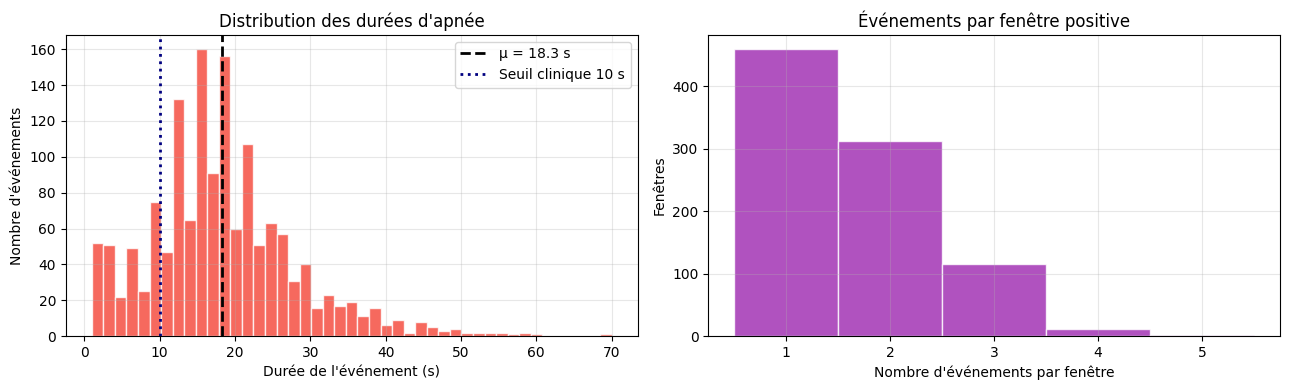
\includegraphics[width=\textwidth,height=3.2cm,keepaspectratio]{fig_09_event_structure.png}
        \end{column}
        \begin{column}{0.46\textwidth}
            \small\textbf{Observations clés}
            \vspace{0.1cm}
            \begin{itemize}\setlength\itemsep{3pt}
                \item Durée moy.\ d'un événement : \textbf{18\,s}
                \item Forte \textbf{variabilité inter-sujets}\\(0\,\% à 70\,\% selon le sujet)
                \item Signaux les plus discriminants :\\AbdoBelt, ThorBelt, AirFlow, SPO2
            \end{itemize}
            \vspace{0.2cm}
            \textcolor{Teal}{\small$\Rightarrow$ Chaque observation justifie un choix de design}
        \end{column}
    \end{columns}
    \vspace{0.1cm}
    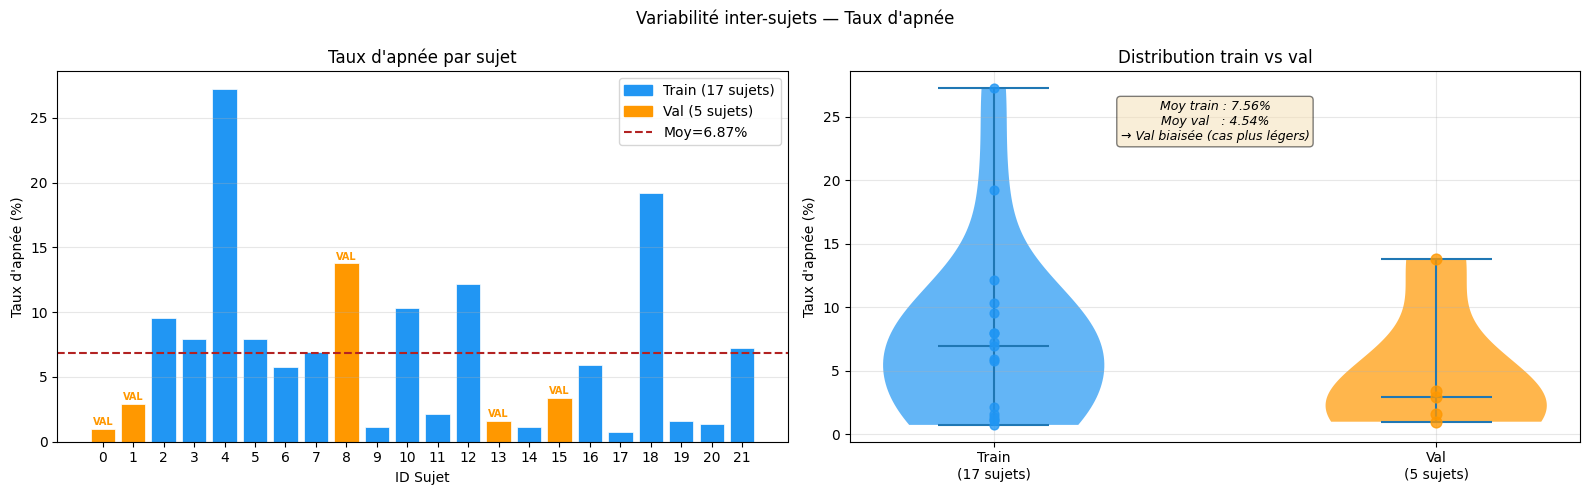
\includegraphics[width=\textwidth,height=2.5cm,keepaspectratio]{fig_03_subject_variability.png}
\end{frame}

% ═════════════════════════════════════════════════════════════════════════════
\section{Métrique}
% ═════════════════════════════════════════════════════════════════════════════

\begin{frame}{F1-score basé sur les événements}
    \begin{columns}[T]
        \begin{column}{0.54\textwidth}
            \small\textbf{Pourquoi pas le F1 pixel-wise ?}\\[2pt]
            On veut détecter des \textbf{événements}, pas prédire chaque seconde.

            \vspace{0.25cm}
            \textbf{Protocole}
            \begin{enumerate}\setlength\itemsep{1pt}\small
                \item Extraire les événements (séquences de 1 consécutifs)
                \item Match si $\displaystyle\text{IoU}(e_p, e_{gt}) =
                      \frac{|e_p \cap e_{gt}|}{|e_p \cup e_{gt}|} \geq 0.3$
                \item $F_1 = \dfrac{2\,\text{TP}}{2\,\text{TP} + \text{FP} + \text{FN}}$
            \end{enumerate}
        \end{column}
        \begin{column}{0.43\textwidth}
            \begin{block}{\small Conséquence}
                \small Un événement prédit \textbf{trop court} ou \textbf{décalé} = FP,
                même si la zone est approximativement bonne.
            \end{block}
            \vspace{0.2cm}
            \begin{alertblock}{\small Benchmark officiel}
                \centering\small CNN 3 couches : \textbf{0.525}
            \end{alertblock}
        \end{column}
    \end{columns}
\end{frame}

% ═══════════════════════════════════════════════════════════════════════════
% PARTIE THÉO — FastDreemTCN
% À insérer après la slide "Métrique" et avant la partie Mateo
% ═══════════════════════════════════════════════════════════════════════════

% ─────────────────────────────────────────────────────────────────────────────
\section{Approche 1 — CNN+BiLSTM : diagnostic de l'overfitting}
% ─────────────────────────────────────────────────────────────────────────────

\begin{frame}{Baseline CNN+BiLSTM — Pourquoi ça ne généralise pas}
    \begin{columns}[T]
        \begin{column}{0.48\textwidth}
            \begin{block}{\small Architecture baseline}
                \small
                \begin{itemize}\setlength\itemsep{2pt}
                    \item 3 blocs Conv1D stride cumulé $\times$100\\
                          $9000 \to 1800 \to 360 \to 90$ pts
                    \item BiLSTM 2 couches bidirectionnel
                    \item Tête linéaire $\to$ 90 logits
                    \item \textbf{261K paramètres}
                \end{itemize}
            \end{block}
            \vspace{0.2cm}
            \begin{alertblock}{\small Résultat}
                \small
                Val F1 = \textbf{0.80} \;\textcolor{Coral}{$\longrightarrow$}\;
                Score public ENS = \textbf{0.447}\\[2pt]
                \textcolor{Coral}{Gap de +0.35 — overfitting massif}
            \end{alertblock}
        \end{column}
        \begin{column}{0.48\textwidth}
            \small\textbf{\textcolor{Coral}{Deux causes cumulées}}
            \vspace{0.15cm}
            \begin{enumerate}\setlength\itemsep{6pt}\small
                \item \textbf{Normalisation globale inadaptée}\\
                      StandardScaler fitté sur 17 sujets train.\\
                      Sujets test : SpO\textsubscript{2} de 74\,\% à 99\,\%\\
                      \textcolor{Coral}{$\to$ features hors distribution au test}

                \item \textbf{Validation biaisée}\\
                      5 sujets val fixes, taux apnée 0.7--2.9\,\%\\
                      (cas les plus légers du dataset)\\
                      \textcolor{Coral}{$\to$ F1 val de 0.80 trop optimiste}
            \end{enumerate}
            \vspace{0.2cm}
            \textcolor{MidGray}{\small
            $\Rightarrow$ Ces deux problèmes sont \textbf{indépendants}\\
            de l'architecture — ils doivent être\\
            corrigés \textit{avant} de changer le modèle.}
        \end{column}
    \end{columns}
\end{frame}

% ─────────────────────────────────────────────────────────────────────────────
\section{Approche 2 — FastDreemTCN}
% ─────────────────────────────────────────────────────────────────────────────

\begin{frame}{Architecture FastDreemTCN — Vue d'ensemble}
    \small
    \[
        (B,\,8,\,9000)
        \;\xrightarrow{\text{CNN réduction }\times 100}\;
        (B,\,128,\,90)
        \;\xrightarrow{\text{TCN dilaté}}\;
        (B,\,128,\,90)
        \;\xrightarrow{\text{Conv}1\times1}\;
        (B,\,90)
    \]

    \vspace{0.15cm}
    \begin{columns}[T]
        \begin{column}{0.50\textwidth}
            \small
            \begin{tabular}{@{}llll@{}}
                \toprule
                \textbf{Étage} & \textbf{Entrée} & \textbf{Sortie} & \textbf{Opération} \\
                \midrule
                CNN Bloc 1 & 9000 pts & 1800 pts & Conv stride=5 \\
                CNN Bloc 2 & 1800 pts & 360 pts  & Conv stride=5 \\
                CNN Bloc 3 & 360 pts  & \textbf{90 pts}   & Conv stride=4 \\
                \midrule
                TCN $d=1$  & 90 pts & 90 pts & CR = 5\,s \\
                TCN $d=2$  & 90 pts & 90 pts & CR = 9\,s \\
                TCN $d=4$  & 90 pts & 90 pts & CR = 17\,s \\
                TCN $d=8$  & 90 pts & 90 pts & CR = 33\,s \\
                \midrule
                Sortie & 90 pts & 90 pts & Conv$1\times1$ \\
                \bottomrule
            \end{tabular}
            \vspace{0.1cm}
            \textcolor{MidGray}{\small CR = champ récepteur effectif}
        \end{column}
        \begin{column}{0.46\textwidth}
            \begin{block}{\small Pourquoi CNN + TCN ?}
                \small
                \textbf{CNN} : réduit $9000 \to 90$ pts\\
                $\to$ une représentation par seconde\\[4pt]
                \textbf{TCN dilaté} : opère sur 90 pts\\
                $\to$ \textbf{10$\times$ plus rapide} qu'un TCN naïf\\[4pt]
                Champ récepteur total : \textbf{61\,s}\\
                Couvre la fenêtre entière de 90\,s\\[4pt]
                $d=4$ cible la durée médiane\\
                d'une apnée (\textbf{17\,s})
            \end{block}
            \vspace{0.1cm}
            \textcolor{MidGray}{\small
            \textbf{458K paramètres}\\
            Forward pass vérifié : $(2,8,9000) \to (2,90)$ \checkmark}
        \end{column}
    \end{columns}
\end{frame}

\begin{frame}{Bloc TCN résiduel — détail}
    \begin{columns}[T]
        \begin{column}{0.50\textwidth}
            \small\textbf{Structure d'un TCNResidualBlock}
            \vspace{0.2cm}

            \begin{tikzpicture}[scale=0.85,
                box/.style={draw, rounded corners=2pt, fill=Teal!10,
                            minimum width=3.2cm, minimum height=0.55cm,
                            font=\small, align=center},
                skip/.style={draw=Coral, thick, ->, dashed}]
                \node[box] (in)   at (0, 0)    {Entrée $(B,128,90)$};
                \node[box] (c1)   at (0,-1.0)  {Conv1d dil=$d$, k=3};
                \node[box] (bn1)  at (0,-1.85) {BatchNorm + ReLU};
                \node[box] (c2)   at (0,-2.7)  {Conv1d dil=$d$, k=3};
                \node[box] (bn2)  at (0,-3.55) {BatchNorm + Dropout};
                \node[box] (add)  at (0,-4.4)  {$+$ Skip \;+\; ReLU};
                \node[box] (out)  at (0,-5.25) {Sortie $(B,128,90)$};

                \draw[->] (in)  -- (c1);
                \draw[->] (c1)  -- (bn1);
                \draw[->] (bn1) -- (c2);
                \draw[->] (c2)  -- (bn2);
                \draw[->] (bn2) -- (add);
                \draw[->] (add) -- (out);
                \draw[skip] (in.east) -- ++(1.1,0) |- (add.east)
                    node[midway, right, font=\tiny, text=Coral] {skip};
            \end{tikzpicture}
        \end{column}
        \begin{column}{0.46\textwidth}
            \begin{block}{\small Convolution dilatée}
                \small Avec dilatation $d$ et kernel $k=3$ :\\[3pt]
                \textbf{Padding} $= d$ $\to$ longueur préservée\\[3pt]
                \textbf{Champ récepteur} d'un bloc :
                \[ \text{CR} = 2(k-1)d + 1 \]
                4 blocs cumulés $(d=1,2,4,8)$ :
                \[ \text{CR}_\text{total} = 61\,\text{pts} = 61\,\text{s} \]
            \end{block}
            \vspace{0.15cm}
            \begin{block}{\small Connexion résiduelle}
                \small Gradient stable même en profondeur\\
                Pas de vanishing gradient\\
                \textcolor{Teal}{Identité si le bloc n'apporte rien}
            \end{block}
        \end{column}
    \end{columns}
\end{frame}

\begin{frame}{Corrections méthodologiques}
    \begin{columns}[T]
        \begin{column}{0.48\textwidth}
            \begin{block}{\small Fix 1 — Instance Normalization}
                \small Par fenêtre et par canal :
                \[
                    \hat{x}_{i,c} =
                    \frac{x_{i,c} - \mu_{i,c}}{\sigma_{i,c} + \varepsilon}
                \]
                Chaque fenêtre normalisée par\\
                \textbf{ses propres statistiques} dans \texttt{\_\_getitem\_\_}\\[4pt]
                Vérification : mean$\approx$0.000, std$\approx$1.001 \checkmark\\[4pt]
                \textcolor{Teal}{Robuste aux sujets test inconnus}\\
                \textcolor{Teal}{Aucun data leakage possible}
            \end{block}
            \vspace{0.15cm}
            \begin{block}{\small Loss — déséquilibre 93/7}
                \small \texttt{BCEWithLogitsLoss(pos\_weight=12.23)}\\
                + Gradient clipping \texttt{max\_norm}=1.0\\
                + Augmentation : bruit $\sigma=0.02$, time shift
            \end{block}
        \end{column}
        \begin{column}{0.48\textwidth}
            \begin{block}{\small Fix 2 — GroupKFold 5 folds}
                \small \textbf{17 sujets train}, 200 fenêtres/sujet
                \vspace{0.1cm}
                \begin{tabular}{@{}ll@{}}
                    \small Fold 1 & val : sujets [3, 9, 16, 21] \\
                    \small Fold 2 & val : sujets [2, 5, 12, 17] \\
                    \small $\vdots$ & $\vdots$ \\
                    \small Fold 5 & val : sujets restants \\
                \end{tabular}
                \vspace{0.1cm}

                Chaque sujet passe \textbf{1 fois} en val\\
                $\to$ 3400 prédictions OOF au total\\[3pt]
                \textcolor{Teal}{F1 OOF = estimateur non biaisé}\\
                \textcolor{Teal}{du score public ENS}
            \end{block}
            \vspace{0.15cm}
            \begin{block}{\small Post-processing}
                \small Filtre médian kernel=5 sur les probabilités\\
                Seuil calibré sur OOF : \textbf{threshold=0.85}
            \end{block}
        \end{column}
    \end{columns}
\end{frame}

\begin{frame}{Calibration du threshold sur prédictions OOF}
    \begin{columns}[T]
        \begin{column}{0.50\textwidth}
            \fbox{\parbox{\textwidth}{\centering\vspace{1.2cm}
            \small\textbf{[SCREENSHOT]}\\
            \texttt{figures/oof\_threshold\_fast\_tcn.png}\\
            Courbe F1-IoU OOF vs threshold\\
            (pic visible à threshold=0.85)
            \vspace{1.2cm}}}
        \end{column}
        \begin{column}{0.46\textwidth}
            \small
            \begin{tabular}{@{}cc@{}}
                \toprule
                \textbf{Threshold} & \textbf{F1-IoU OOF} \\
                \midrule
                0.10 & 0.573 \\
                0.30 & 0.727 \\
                0.50 & 0.787 \\
                0.70 & 0.818 \\
                \textbf{0.85} & \textbf{0.831} $\leftarrow$ optimal \\
                \bottomrule
            \end{tabular}
            \vspace{0.25cm}
            \begin{block}{\small Pourquoi threshold = 0.85 ?}
                \small \texttt{pos\_weight=12.23} pousse le modèle\\
                à prédire des probabilités élevées\\
                pour les apnées.\\[3pt]
                Un seuil haut élimine les\\
                faux positifs de faible confiance.\\[3pt]
                \textcolor{Teal}{Calibré sur OOF $\to$ pas de leakage}
            \end{block}
        \end{column}
    \end{columns}
\end{frame}

\begin{frame}{Résultats FastDreemTCN}
    \begin{columns}[T]
        \begin{column}{0.50\textwidth}
            \fbox{\parbox{\textwidth}{\centering\vspace{1.2cm}
            \small\textbf{[SCREENSHOT]}\\
            \texttt{figures/fold\_f1\_fast\_tcn.png}\\
            Barplot F1 par fold\\
            + ligne F1 OOF moyen
            \vspace{1.2cm}}}
        \end{column}
        \begin{column}{0.46\textwidth}
            \small
            \begin{tabular}{@{}lcc@{}}
                \toprule
                \textbf{} & \textbf{Val F1} & \textbf{Public} \\
                \midrule
                CNN+BiLSTM   & 0.80 \textcolor{Coral}{(biaisé)} & 0.447 \\
                \midrule
                FastDreemTCN & & \\
                \quad Fold 1 & 0.63 & --- \\
                \quad Fold 2 & --- & --- \\
                \quad $\vdots$ & & \\
                \quad OOF moy. & \textbf{0.83} & --- \\
                \midrule
                \textbf{Score ENS} & --- & \textbf{0.5895} \\
                \bottomrule
            \end{tabular}
            \vspace{0.2cm}
            \begin{alertblock}{\centering\small Score final}
                \centering\normalsize\textbf{F1 = 0.5895}\\
                \small $+12\,\%$ vs benchmark (0.525)\\
                $+0.14$ vs CNN+BiLSTM baseline
            \end{alertblock}
            \vspace{0.1cm}
            \small\textbf{Sanity check :}\\
            \% apnées test = 8.41\,\% vs 7.56\,\% train\\
            Ratio = 1.11 \textcolor{Teal}{\checkmark}
        \end{column}
    \end{columns}
\end{frame}

% ═════════════════════════════════════════════════════════════════════════════
% ── PARTIE MATEO ─────────────────────────────────────────────────────────────
% ═════════════════════════════════════════════════════════════════════════════

\section{Approche 3 --- Attention U-Net 1D (Mateo)}

\begin{frame}{Attention U-Net 1D}
    \small Input $(B,\,8,\,9000)$ à 100\,Hz $\;\longrightarrow\;$ Output $(B,\,90)$ à 1\,Hz

    \vspace{0.2cm}
    \begin{columns}[T]
        \begin{column}{0.50\textwidth}
            \small
            \begin{tabular}{@{}lll@{}}
                \toprule
                \textbf{Étage} & \textbf{Résol.} & \textbf{Opération} \\
                \midrule
                Encodeur 1   & 100\,Hz & ConvBlock ($F$) \\
                Encodeur 2   & 10\,Hz  & Pool$\!\times\!10$ + CB ($2F$) \\
                Bottleneck   & 1\,Hz   & Pool$\!\times\!10$ + Dilatés ($4F$) \\
                Décodeur     & 10\,Hz  & Upsample + \textcolor{Teal}{Attn} \\
                Sortie       & 1\,Hz   & Pool$\!\times\!10$ + Conv$1\!\times\!1$ \\
                \bottomrule
            \end{tabular}
            \vspace{0.15cm}

            \textcolor{MidGray}{\small $F = 64$ filtres --- \textbf{3\,M paramètres}}

            \vspace{0.2cm}
            \small\textbf{ConvBlock} = Conv--BN--GELU $\times$ 2 + résiduelle\\
            \textbf{Bottleneck dilaté} : dilatations 1, 2, 4
        \end{column}
        \begin{column}{0.46\textwidth}
            \begin{block}{\small Attention Gate}
                \small Filtre les skip connections selon le contexte global :
                \[
                    \alpha = \sigma\!\bigl(\psi(\text{GELU}(W_g g + W_x x))\bigr)
                \]
                \textcolor{Teal}{$\Rightarrow$ focalise sur les zones d'apnée}
            \end{block}
            \vspace{0.15cm}
            \begin{block}{\small Pourquoi U-Net ?}
                \small Segmentation 1D = analogue à la segmentation d'image biomédicale.
                Les skip connections préservent la résolution temporelle fine.
            \end{block}
        \end{column}
    \end{columns}
\end{frame}

% ═════════════════════════════════════════════════════════════════════════════
\section{Pipeline d'entraînement}
% ═════════════════════════════════════════════════════════════════════════════

\begin{frame}{Prétraitement \& Loss}
    \begin{columns}[T]
        \begin{column}{0.48\textwidth}
            \begin{block}{\small Normalisation instance}
                \small Par fenêtre et par canal :
                $\hat{x}_{i,c} = \frac{x_{i,c} - \mu_{i,c}}{\sigma_{i,c} + \varepsilon}$\\[2pt]
                Supprime la baseline inter-sujets.\\
                \textcolor{Teal}{\textbf{+0.065 de F1 sur le test}}
            \end{block}
            \vspace{0.15cm}
            \begin{block}{\small Augmentation}
                \small Scaling $U(0.85,1.15)$,\;
                bruit $\mathcal{N}(0,0.02^2)$,\;
                channel dropout $p\!=\!0.05$
            \end{block}
        \end{column}
        \begin{column}{0.48\textwidth}
            \begin{block}{\small Loss combinée --- déséquilibre 93/7}
                \small $\mathcal{L} = 0.5\,\mathcal{L}_{\text{BCE}}^{w=10}
                                     + 0.5\,\mathcal{L}_{\text{Dice}}$
                \begin{itemize}\setlength\itemsep{1pt}\small
                    \item BCE : pénalise $10\times$ les faux négatifs
                    \item Dice : optimise l'IoU, invariante au déséquilibre
                \end{itemize}
            \end{block}
            \vspace{0.15cm}
            \begin{block}{\small Optimisation}
                \small AdamW, lr$=10^{-3}$, wd$=10^{-3}$,
                12 epochs, batch 32, grad clip 1.0
            \end{block}
        \end{column}
    \end{columns}
\end{frame}

\begin{frame}{Post-traitement \& Calibration OOF}
    \begin{columns}[T]
        \begin{column}{0.48\textwidth}
            \begin{block}{\small Post-traitement}
                \small Supprimer les événements prédits $<\mathbf{10\,s}$\\[2pt]
                \textbf{Justification EDA :} durée min réelle $\approx5$\,s, moy 18\,s\\
                $\Rightarrow$ prédictions courtes $\approx$ faux positifs\\[2pt]
                \textcolor{Teal}{\textbf{+0.076 --- gain le plus important}}
            \end{block}
        \end{column}
        \begin{column}{0.48\textwidth}
            \begin{block}{\small 5-fold GroupKFold --- sans data leakage}
                \small
                \begin{enumerate}\setlength\itemsep{1pt}
                    \item 5 modèles entraînés sur $\approx$18 sujets
                    \item Prédictions OOF sur les sujets exclus
                    \item Grid search \{threshold, min\_dur\}\\
                          sur les 4400 prédictions OOF
                \end{enumerate}
                \textcolor{Teal}{Aucun sujet vu à l'entraînement}\\
                \textcolor{Teal}{ne contribue à la calibration}
            \end{block}
        \end{column}
    \end{columns}
\end{frame}

% ═════════════════════════════════════════════════════════════════════════════
\section{Résultats}
% ═════════════════════════════════════════════════════════════════════════════

\begin{frame}{Progression des scores}
    \begin{columns}[T]
        \begin{column}{0.50\textwidth}
            \fbox{\parbox{\textwidth}{\centering\vspace{1.4cm}
            \small\textbf{[SCREENSHOT]}\\
            Section 8 notebook :\\
            Barplot F1 par version\\
            + ligne benchmark 0.525
            \vspace{1.4cm}}}
        \end{column}
        \begin{column}{0.46\textwidth}
            \small
            \begin{tabular}{@{}lcc@{}}
                \toprule
                \textbf{Version} & \textbf{F1} & \textbf{$\Delta$} \\
                \midrule
                Benchmark CNN       & 0.525 & ---  \\
                U-Net baseline      & 0.473 & ---  \\
                + Post-proc.        & 0.549 & \textcolor{Teal}{+.076} \\
                + Inst.\ norm.      & 0.614 & \textcolor{Teal}{+.065} \\
                + Tous sujets       & 0.624 & \textcolor{Teal}{+.010} \\
                + $F\!=\!64$        & 0.630 & \textcolor{Teal}{+.006} \\
                \textbf{+ thr=0.70} & \textbf{0.636} & \textcolor{Teal}{\textbf{+.006}} \\
                \bottomrule
            \end{tabular}
            \vspace{0.2cm}
            \begin{alertblock}{\centering\small Score final}
                \centering\normalsize\textbf{0.636} \;\;$+21\,\%$ vs benchmark
            \end{alertblock}
            \begin{exampleblock}{\centering\small Leaderboard}
                \centering\small \textbf{3\textsuperscript{e}} \;|\;
                leo\_h 0.670 $\cdot$ clementg 0.650
            \end{exampleblock}
        \end{column}
    \end{columns}
\end{frame}

\begin{frame}{Exemples de prédictions}
    \fbox{\parbox{\textwidth}{\centering\vspace{1.5cm}
    \textbf{[SCREENSHOT]}\\
    Section 7 notebook : grille 2$\times$3 de fenêtres\\
    Probabilités prédites (rouge) vs labels réels (vert) + seuil (pointillés)
    \vspace{1.5cm}}}
\end{frame}

% ═════════════════════════════════════════════════════════════════════════════
\section{Discussion}
% ═════════════════════════════════════════════════════════════════════════════

\begin{frame}{Comparaison des deux approches}
    \small
    \begin{tabular}{@{}lccc@{}}
        \toprule
        \textbf{Aspect} & \textbf{CNN+BiLSTM} & \textbf{FastDreemTCN} & \textbf{Attn U-Net} \\
        \midrule
        Architecture      & CNN + LSTM      & CNN + TCN dilaté    & U-Net + Attention \\
        Paramètres        & 261K            & 290K                & 3M \\
        Normalisation     & Globale         & Instance            & Instance \\
        Validation        & Split biaisé    & GroupKFold 5F       & GroupKFold 5F \\
        Loss              & BCE             & BCE                 & BCE + Dice \\
        Post-proc.        & Médian k=5      & Médian k=5          & Suppression $<$10s \\
        \midrule
        \textbf{Score public} & 0.36 & 0.5895 & \textbf{0.636} \\
        \bottomrule
    \end{tabular}
    \vspace{0.25cm}
    \begin{columns}[T]
        \begin{column}{0.48\textwidth}
            \begin{block}{\small Convergence méthodologique}
                \small Instance norm + GroupKFold\\
                validés indépendamment par les deux approches\\
                \textcolor{Teal}{$\to$ résultats cohérents et robustes}
            \end{block}
        \end{column}
        \begin{column}{0.48\textwidth}
            \begin{alertblock}{\small Écart résiduel (0.047)}
                \small U-Net : skip connections + Dice loss\\
                $\to$ meilleure segmentation des bords\\
                \textcolor{Coral}{au coût de 10$\times$ plus de paramètres}
            \end{alertblock}
        \end{column}
    \end{columns}
\end{frame}

\begin{frame}{Limites \& Perspectives}
    \begin{columns}[T]
        \begin{column}{0.48\textwidth}
            \textbf{\textcolor{Coral}{Limites}}
            \begin{itemize}\setlength\itemsep{3pt}\small
                \item \textbf{22 sujets} --- overfitting inter-sujet inévitable
                \item \textbf{Désalignement loss/métrique} ---
                      BCE+Dice $\neq$ F1 événementiel,\\
                      nécessite post-processing
                \item Hétérogénéité des folds (F1 entre 0.50 et 0.62)
            \end{itemize}
        \end{column}
        \begin{column}{0.48\textwidth}
            \textbf{\textcolor{Teal}{Perspectives}}
            \begin{itemize}\setlength\itemsep{3pt}\small
                \item \textbf{Ensemble} des 5 modèles CV
                \item \textbf{Test-Time Augmentation}
                \item \textbf{Loss event-aware} ---
                      optimiser directement le F1 cible
                \item \textbf{Transformer 1D} ---
                      dépendances longue portée
            \end{itemize}
        \end{column}
    \end{columns}
\end{frame}

% ── CONCLUSION ────────────────────────────────────────────────────────────────
{
\setbeamercolor{background canvas}{bg=DarkNavy}
\begin{frame}[standout]
    \color{white}\centering
    \large\textbf{Conclusion}\normalsize\\[0.8em]
    \begin{tabular}{@{}r@{\quad}l@{}}
        \textbf{FastDreemTCN} & CNN réduction + TCN dilaté --- 290K paramètres \\[3pt]
        Clé \#1  & Instance normalization \textcolor{Teal}{(généralise aux sujets test)} \\[3pt]
        Clé \#2  & GroupKFold 5 folds \textcolor{Teal}{(validation honnête)} \\[3pt]
        Score    & \textcolor{Teal}{\textbf{F1 = 0.5895}} \quad $+12\,\%$ vs benchmark \\[10pt]
        \textbf{Attention U-Net} & U-Net 1D + Attention Gates --- 3M paramètres \\[3pt]
        Clé \#1  & Post-traitement durée min \textcolor{Teal}{(+0.076)} \\[3pt]
        Clé \#2  & Instance norm + Dice loss \textcolor{Teal}{(+0.065)} \\[3pt]
        Score    & \textcolor{Teal}{\textbf{F1 = 0.636 --- 3\textsuperscript{e} du leaderboard}}
    \end{tabular}
    \vspace{0.5em}
    \textcolor{MidGray}{\small Merci}
\end{frame}
}

\end{document}